\documentclass[12pt,a4paper]{report}

% -------------------------------------------------
% Packages
% -------------------------------------------------
\usepackage[a4paper,margin=1in]{geometry}
\usepackage{fontspec}
\setmainfont{Times New Roman}
\usepackage{setspace}
\usepackage{amsmath,amssymb,amsfonts}
\usepackage{graphicx}
\usepackage{float}
\usepackage{booktabs}
\usepackage{array}
\usepackage{longtable}
\usepackage{multirow}
\usepackage{caption}
\usepackage{subcaption}
\usepackage{titlesec}
\usepackage{fancyhdr}
\usepackage{tocloft}
\usepackage{xcolor}
\usepackage{enumitem}
\usepackage{verbatim}
\usepackage{tikz}
\usepackage{tabularx}
\usepackage{microtype}
\usepackage[normalem]{ulem}
\usepackage{listings}
\usetikzlibrary{calc}
\usepackage[hidelinks]{hyperref}

% -------------------------------------------------
% Formatting
% -------------------------------------------------
\onehalfspacing
\setlength{\parindent}{0pt}
\setlength{\parskip}{0.5em}
\setcounter{secnumdepth}{3}
\setcounter{tocdepth}{2}

\hypersetup{
    colorlinks=false,
    pdftitle={IndustrialSensorMonitoring Communication},
    pdfauthor={KLH University},
    pdfsubject={Project Report},
    pdfkeywords={BPSK, industrial monitoring, Python, communication system}
}
\pagestyle{fancy}
\fancyhf{}
\fancyhead[L]{Mathematics for Communication Systems}
\fancyhead[R]{25MT1307E}
\fancyfoot[L]{Batch 9}
\fancyfoot[C]{\thepage}
\renewcommand{\headrulewidth}{0.4pt}
\renewcommand{\footrulewidth}{0.4pt}
\setlength{\headheight}{14.5pt}

\fancypagestyle{plain}{%
  \fancyhf{}
  \fancyhead[L]{Mathematics for Communication Systems}
  \fancyhead[R]{25MT1307E}
  \fancyfoot[R]{Batch 9}
  \fancyfoot[C]{\thepage}
  \renewcommand{\headrulewidth}{0.4pt}
  \renewcommand{\footrulewidth}{0.4pt}
}

\titleformat{\chapter}[display]
  {\bfseries\Large}
  {\chaptername\ \thechapter}{10pt}{\Large}

% -------------------------------------------------
% Listings style
% -------------------------------------------------
\lstdefinestyle{pythonstyle}{
    language=Python,
    basicstyle=\ttfamily\small,
    keywordstyle=\color{blue},
    commentstyle=\color{green!40!black},
    stringstyle=\color{red!60!black},
    numbers=left,
    numberstyle=\tiny,
    stepnumber=1,
    numbersep=8pt,
    breaklines=true,
    breakatwhitespace=true,
    showstringspaces=false,
    frame=single,
    tabsize=4,
    captionpos=b
}
\lstset{style=pythonstyle}

% -------------------------------------------------
% Document
% -------------------------------------------------
\begin{document}

\pagenumbering{roman}

% Front matter
\begin{titlepage}
    \thispagestyle{empty}
    \newgeometry{left=0.9cm,right=0.9cm,top=0.7cm,bottom=0.7cm}
    
    \begin{tikzpicture}[remember picture,overlay]
    \draw[line width=2.25pt,black]
    ($(current page.north west)+(0.6cm,-0.6cm)$) rectangle
    ($(current page.south east)+(-0.6cm,0.6cm)$);
    \end{tikzpicture}
    
    \vspace*{0.15cm}
    
    \begin{center}
        
\includegraphics[width=3.6cm]{assets/logo.jpg}
    
        \vspace{0.18cm}
        {\large Department of Electronics and Communication Engineering\par}
        \vspace{0.05cm}
        {\bfseries\Large PROJECT REPORT\par}
    
        \vspace{0.18cm}
        {\bfseries Course Name: Mathematics for Communication Systems\par}
        {\bfseries Course Code: 25MT1307E\par}
    
        \vspace{0.18cm}
        \hrule
        \vspace{0.16cm}
    
        {\bfseries\large Design and Simulation of Industrial Sensor Monitoring Communication Using BPSK and Python.\par}
    
        \vspace{0.16cm}
        \hrule
    \end{center}
    
    \vspace{0.25cm}
    
    {\bfseries Submitted by:\par}
    \vspace{0.10cm}
    
    \renewcommand{\arraystretch}{1.1}
    \begin{tabularx}{\textwidth}{@{}>{\bfseries}p{4.6cm}X@{}}
    Name of Student 1: & Challa Deepak Sai Kumar Reddy \\
    Registration No: & 2520040041 \\
    Name of Student 2: & Bikkina Vijay Ganesh Koushik Chandar \\
    Registration No: & 2520040054 \\
    Name of Student 3: & Kanuri Sri Ram \\
    Registration No: & 2520040072 \\
    Name of Student 4: & Koppolu Bhargava Aditya \\
    Registration No: & 2520040077 \\
    \end{tabularx}
    
    \vspace{0.15cm}
    
    \begin{tabularx}{\textwidth}{@{}>{\bfseries}p{4.6cm}X@{}}
    Batch Number: & 9 \\
    Application Theme: &  Remote Industrial Sensor Monitoring and Reliable Data Communication\\
    \end{tabularx}
    
    \vspace{0.15cm}
    
    {\bfseries Submitted to:\par}
    \vspace{0.05cm}
    
    \begin{tabularx}{\textwidth}{@{}>{\bfseries}p{4.6cm}X@{}}
    Course Instructor: & B.Praveen Sai \\
    \end{tabularx}
    
    \vfill
    
    \begin{center}
        {\bfseries Academic Year: 2025--2026\par}
        {\bfseries Term: 3\par}
    \end{center}
    
    \restoregeometry
\end{titlepage}

\clearpage
\chapter*{Certificate}
\addcontentsline{toc}{chapter}{Certificate}

This is to certify that the project report entitled 
\textbf{\textit{Design and Simulation of Industrial Sensor Monitoring Communication Using BPSK and Python}}, 
submitted by the students listed on the title page, is a bonafide record of project work carried out as part of the course 
\textbf{\textit{Mathematics for Communication Systems}}, Course Code
\textbf{\textit{25MT1307E}},
 during the academic year 
\textbf{\textit{2025--2026}}.

The project has been implemented using Python/Jupyter Notebook and addresses the required course outcomes from 
\textbf{\textit{CO1}} to \textbf{\textit{CO6}},through mathematical modeling, simulation, analysis, and interpretation of a BPSK-based digital communication system.

\vspace{2.5cm}

\begin{flushright}
\textbf{Signature of Course Instructor}
\end{flushright}

\clearpage
\clearpage
\chapter*{Declaration}
\addcontentsline{toc}{chapter}{Declaration}

We hereby declare that the project work presented in this report is our original work carried out as part of the course 
\textbf{\textit{Mathematics for Communication Systems}}
The Python code, plots, analysis, mathematical derivations, and conclusions included in this report have been prepared by our team using the assigned Batch 9 parameters for the given application theme.

We further declare that proper academic care has been taken to maintain originality in ~\\
implementation, analysis, and presentation. All numerical results, waveform plots, BER curves, receiver outputs, and capacity-related observations are produced specifically for the assigned specifications and are not copied from any other batch submission.

\vspace{1.8cm}

\begin{flushleft}
\textbf{Student Signatures:}\\[0.8cm]
1.\underline{\hspace{6cm}}\\
2.\underline{\hspace{6cm}}\\
3.\underline{\hspace{6cm}}\\
4.\underline{\hspace{6cm}}\\
\end{flushleft}

\clearpage
\clearpage
\chapter*{Acknowledgement}
\addcontentsline{toc}{chapter}{Acknowledgement}

\sloppy express our sincere gratitude to 
our course instructor and course coordinator 
for their valuable guidance, encouragement, 
and continuous support throughout the completion of this project.

This work gave us an opportunity to understand the mathematical foundations of communication systems through practical Python implementation. By carrying out this project, we were able to connect theoretical concepts such as signal representation, Fourier analysis, channel modeling, matched filtering, probability-based error analysis, and Shannon capacity with a meaningful engineering application.

We also extend our thanks to the Department of Electronics and Communication Engineering, KLH University, for providing the academic environment and support required for the
\\successful completion of this report.

\clearpage
\clearpage
\chapter*{Abstract}
\addcontentsline{toc}{chapter}{Abstract}

This project presents the complete development and analysis of a Binary Phase Shift Keying (BPSK) based digital communication system using Python for the application theme \textit{Industrial Sensor Monitoring Communication}. The work models a practical sensor-data transmission link in which binary information generated by an industrial monitoring node is conveyed to a nearby receiver through a noisy wireless channel.

The implementation includes BPSK symbol generation, energy-per-bit calculation,
generation of a 10-bit transmitted waveform, Fourier spectrum analysis, 
power spectral density estimation, null-to-null bandwidth evaluation, 
and Parseval verification. In accordance with the assigned
 specifications, the communication channel is modeled as a mild low-pass channel followed by additive white Gaussian noise.

At the receiver, both a correlator detector and an FIR matched filter detector are implemented and compared. 
The project further includes Monte Carlo bit error rate simulation, comparison with the theoretical BER expression for BPSK,
Shannon capacity evaluation, and discussion of the performance gap between uncoded BPSK and the Shannon limit.

The main objective of this work is to connect mathematical ideas from signals and systems, probability, transforms, LTI systems, and information theory with a practical digital
\\communication design problem. The results are supported through numerical calculations,\\
simulation outputs, and graphical interpretation.


\clearpage
\clearpage
\chapter*{Keywords}
\addcontentsline{toc}{chapter}{Keywords}

\textbf{Keywords:} BPSK, Industrial Sensor Monitoring Communication, Mild Low-Pass Channel, AWGN, Correlator Receiver, FIR Matched Filter, Bit Error Rate, Shannon Capacity, Python, Communication Systems.

\clearpage
\clearpage

% Tables and lists
\tableofcontents
\clearpage
\listoffigures
\clearpage
\listoftables
\clearpage

\pagenumbering{arabic}

% Chapters
\chapter{Introduction}

\section{Background}
Digital communication systems are widely used in modern monitoring and control applications 
where sensor data must be transmitted reliably from a sensing node to a receiver. 
In industrial environments, sensors are commonly deployed to monitor parameters 
such as temperature, \\vibration, pressure, gas concentration, flow rate, and machine health. 
These measurements are often converted into binary form and sent through a communication link for further processing, logging, or control action.

In this project, the selected application theme is 
\textbf{\textit{Industrial Sensor Monitoring \\Communication}}. 
In such a scenario, an industrial sensor node generates binary information and transmits it wirelessly to a nearby receiver. 
Because practical transmission channels are affected by \\attenuation, distortion, and noise, the received signal may differ from the transmitted signal. 
Hence, proper modulation and receiver design are essential for reliable data recovery.

Binary Phase Shift Keying (BPSK) is one of the simplest and most reliable digital modulation techniques for binary data transmission. 
In BPSK, bit `1` and bit `0` are represented by two antipodal carrier waveforms having a phase difference of \(180^\circ\). 
Due to its simple structure and strong noise tolerance, 
BPSK is widely used as a basic model for understanding digital communication theory.

The present work studies a complete BPSK communication chain using mathematical analysis and Python simulation. 
The work includes waveform generation, energy calculation, Fourier-domain analysis, bandwidth estimation, channel modeling, correlator detection, FIR matched filter implementation, BER simulation, and Shannon-capacity interpretation. 
Since assigned a mild low-pass channel followed by AWGN and both receiver types, this report gives special attention to channel distortion and detector comparison.

\section{Project Objective}
The main objective of this project is to develop a complete BPSK-based communication link in Python for the assigned industrial monitoring scenario 
and to analyse its performance using the mathematical concepts covered in the course.

The specific objectives of this project are listed below:
\begin{enumerate}[label=\arabic*.]
    \item To generate the BPSK symbols corresponding to binary `1` and binary `0` using the \\assigned carrier frequency, bit rate, and sampling frequency.
    \item To compute the bit duration, samples per bit, and energy per bit, and to compare numerical and theoretical energy values.
    \item To generate and visualize the transmitted 10-bit BPSK waveform for the prescribed test bit sequence.
    \item To analyse the FFT spectrum, power spectral density, bandwidth, and Parseval relation of the generated signal.
    \item To model the assigned transmission channel, namely a mild low-pass channel followed by additive white Gaussian noise.
    \item To implement and compare both a correlator receiver and an FIR matched filter receiver.
    \item To perform Monte Carlo BER simulation and compare simulated BER with the theoretical BER expression of BPSK.
    \item To compute Shannon channel capacity and discuss the gap between uncoded BPSK \\performance and the Shannon limit.
\end{enumerate}

\section{Course Outcome Coverage}

\begin{table}[H]
\centering
\caption{CO-wise project coverage}
\begin{tabular}{|c|p{0.75\linewidth}|}
\hline
\textbf{CO} & \textbf{Project Component} \\
\hline
CO1 & BPSK signal representation, sinusoidal modeling, antipodal signaling, and energy-per-bit calculation. \\
\hline
CO2 & Fourier spectrum analysis, power spectral density estimation, bandwidth calculation, and Parseval verification. \\
\hline
CO3 & Mild low-pass channel modeling, AWGN inclusion, convolution, and correlator receiver design. \\
\hline
CO4 & Sampled-signal processing, FIR matched filter design, stability discussion, and discrete-time interpretation using Z-transform ideas. \\
\hline
CO5 & Q-function based theoretical BER, random-bit generation, Monte Carlo BER simulation, and practical detector validation. \\
\hline
CO6 & Shannon capacity calculation, spectral-efficiency discussion, and comparison between practical uncoded BPSK and the Shannon limit. \\
\hline
\end{tabular}
\end{table}
\chapter{Assigned Batch Parameters}

\section{Application Scenario}
This project considers an industrial sensor monitoring communication system in which a \\remote sensor node measures process variables 
such as temperature, vibration, pressure, or \\machine health condition and transmits the data wirelessly to a nearby monitoring receiver. 
The transmitted information is represented in binary form and modulated using Binary Phase Shift Keying (BPSK), 
which is selected because of its simple implementation and reliable \\performance in noisy environments.

For our batch, the communication channel is modeled as a mild low-pass channel followed by additive white Gaussian noise (AWGN). 
At the receiver side, both the correlator receiver and the FIR matched filter receiver are implemented and compared in order 
to study their detection performance under the assigned channel condition.

\section{Numerical Specifications}
The batch-specific numerical parameters assigned for this project are listed in Table~\ref{tab:batch9params}. 
These values are used throughout the Python implementation, simulation, and analysis.

\begin{table}[H]
\centering
\caption{Assigned numerical parameters}
\label{tab:batch9params}
\begin{tabular}{|l|l|}
\hline
\textbf{Parameter} & \textbf{Assigned Value} \\
\hline
Application theme & Industrial Sensor Monitoring Communication \\
\hline
Carrier frequency, \(f_c\) & 15 kHz \\
\hline
Bit rate, \(R_b\) & 1 kbps \\
\hline
Bit duration, \(T_b = 1/R_b\) & 1 ms \\
\hline
Sampling frequency, \(f_s\) & 200 kHz \\
\hline
Samples per bit, \(N = f_s/R_b\) & 200 \\
\hline
Signal amplitude, \(A\) & 1 V \\
\hline
Number of bits for BER simulation & \(10^5\) \\
\hline
\(E_b/N_0\) range & 2 dB to 14 dB \\
\hline
Channel type & Mild LPF + AWGN \\
\hline
Low-pass channel impulse response & \(h[n] = [0.2,\;0.6,\;0.2]\) \\
\hline
Receiver type & Both correlator and FIR matched filter \\
\hline
Decision threshold & 0 \\
\hline
\end{tabular}
\end{table}

\section{Derived Quantities}
From the assigned numerical values, a few important derived quantities are calculated and used in later chapters. 
These quantities help in waveform generation, spectrum analysis, and receiver implementation.

The bit duration is
\[
T_b = \frac{1}{R_b} = \frac{1}{1000} = 0.001~\text{s} = 1~\text{ms}
\]

The number of samples per bit is
\[
N = \frac{f_s}{R_b} = \frac{200000}{1000} = 200
\]

The theoretical energy per bit for BPSK is
\[
E_b = \frac{A^2 T_b}{2}
\]
Since \(A = 1\) V and \(T_b = 0.001\) s,
\[
E_b = \frac{(1)^2 \times 0.001}{2} = 0.0005~\text{J}
\]

The null-to-null bandwidth of BPSK is
\[
BW = 2R_b = 2 \times 1000 = 2000~\text{Hz}
\]

The first spectral null frequencies are
\[
f_{\text{lower null}} = f_c - R_b = 15000 - 1000 = 14000~\text{Hz}
\]
\[
f_{\text{upper null}} = f_c + R_b = 15000 + 1000 = 16000~\text{Hz}
\]

These values are important because they define the expected frequency-domain shape of the transmitted BPSK signal and help validate the FFT and PSD plots.

\section{Discussion}
The assigned parameter set corresponds to a practical low-data-rate industrial monitoring link, where reliable transmission is more important than very high speed. 
The presence of a mild low-pass channel makes the problem more realistic because real industrial links often introduce slight distortion in addition to random noise.

Since both correlator and matched filter receivers are assigned, this batch provides a good \\opportunity to compare the two detection methods and verify their equivalence in decision \\making. 
The BER and capacity results obtained later in the report will therefore reflect both \\theoretical understanding and practical simulation performance.
\chapter{BPSK Signal Generation and Energy Analysis}
\section{Mathematical Representation}
For BPSK, the bit 1 and bit 0 waveforms are represented as
\[s_1(t) = A \cos(2\pi f_c t)\]\[s_0(t) = -A \cos(2\pi f_c t)\]
where \(A\) is the signal amplitude and \(f_c\) is the carrier frequency.
For the assigned values, we have
\[
A = 1~\text{V}, \quad f_c = 15~\text{kHz}, \quad R_b = 1~\text{kbps}, \quad f_s = 200~\text{kHz}
\]

The bit duration is
\[
T_b = \frac{1}{R_b} = 1~\text{ms}
\]
and the samples per bit are
\[
N = \frac{f_s}{R_b} = 200
\]

\section{Energy Per Bit}
The energy per bit is given by
\[
E_b = \int_0^{T_b} s^2(t)\,dt
\]
For a cosine BPSK waveform, the theoretical energy per bit becomes
\[
E_b = \frac{A^2 T_b}{2}
\]
Substituting the assigned values,
\[
E_b = \frac{(1)^2 \times 0.001}{2} = 0.0005~\text{J}
\]

\section{Python Implementation}
The following Python code generates the one-bit BPSK symbols and verifies the energy \\calculation.

\begin{lstlisting}[style=pythonstyle, caption={BPSK Symbol Generation and Energy Calculation}]
    import numpy as np
    import matplotlib.pyplot as plt
    
    A = 1
    fc = 15000
    Rb = 1000
    fs = 200000
    
    Tb = 1 / Rb
    N = int(fs / Rb)
    t = np.arange(0, Tb, 1/fs)
    s1 = A * np.cos(2 * np.pi * fc * t)
    s0 = -A * np.cos(2 * np.pi * fc * t)
    
    Eb_num = np.sum(s1**2) / fs
    Eb_theory = (A**2 * Tb) / 2

    print("Numerical Eb =", Eb_num)
    print("Theoretical Eb =", Eb_theory)
    
    plt.figure(figsize=(8,4))
    plt.plot(t, s1, label='Bit 1')
    plt.plot(t, s0, label='Bit 0', linestyle='--')
    plt.xlabel('Time (s)')
    plt.ylabel('Amplitude (V)')
    plt.title('BPSK Symbols for Bit 1 and Bit 0')
    plt.grid(True)
    plt.legend()
    plt.tight_layout()
    plt.show()
    \end{lstlisting}

\section{Results and Discussion}
The two waveforms are antipodal, which means they have equal magnitude and opposite phase. This property is what makes BPSK simple and robust for binary data transmission.

The numerical energy per bit should be very close to the theoretical value \(0.0005\) J. A very small difference, if present, is due to finite sampling in the numerical integration.

\begin{figure}[htbp]
    \centering
    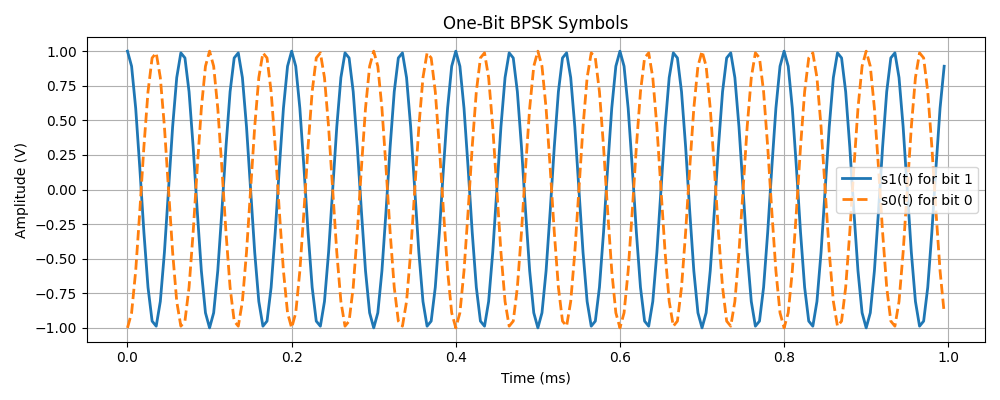
\includegraphics[width=0.8\textwidth]{plots/bpsk.png}
    \caption{BPSK plot}
    \end{figure}
\chapter{BPSK Waveform Generation}

\section{Input Bit Sequence}
For waveform visualization, the assigned 10-bit sequence is
\[
1,\,0,\,1,\,1,\,0,\,0,\,1,\,0,\,1,\,0
\]

This sequence is used to generate the complete transmitted BPSK waveform by concatenating the one-bit BPSK symbols.

\section{Python Implementation}
The following Python code generates the 10-bit BPSK waveform and marks the bit boundaries on the plot.

\begin{lstlisting}[style=pythonstyle, caption={10-Bit BPSK Waveform Generation}]
import numpy as np
import matplotlib.pyplot as plt

A = 1
fc = 15000
Rb = 1000
fs = 200000

Tb = 1 / Rb
N = int(fs / Rb)
t_bit = np.arange(0, Tb, 1/fs)

s1 = A * np.cos(2 * np.pi * fc * t_bit)
s0 = -A * np.cos(2 * np.pi * fc * t_bit)

bits = np.array([1,0,1,1,0,0,1,0,1,0])
waveform = np.array([])

for bit in bits:
    if bit == 1:
        waveform = np.concatenate((waveform, s1))
    else:
        waveform = np.concatenate((waveform, s0))

timeaxis = np.arange(len(waveform)) / fs

plt.figure(figsize=(12,4))
plt.plot(timeaxis, waveform, linewidth=1.2)
for k in range(len(bits) + 1):
    plt.axvline(k * Tb, color='red', linestyle='--', linewidth=0.8)

plt.xlabel('Time (s)')
plt.ylabel('Amplitude (V)')
plt.title('10-Bit BPSK Waveform')
plt.grid(True)
plt.tight_layout()
plt.show()
\end{lstlisting}

\section{Results and Discussion}
The generated waveform shows how binary data is carried using phase changes of the same cosine carrier. A bit value of 1 is represented by a cosine wave, while a bit value of 0 is represented by the same wave with 180-degree phase reversal.

The vertical dashed lines indicate bit boundaries, so it becomes easy to see where each bit starts and ends. Whenever the bit changes from 1 to 0 or 0 to 1, the waveform flips its phase, which is the main visual signature of BPSK.

\begin{figure}[htbp]
    \centering
    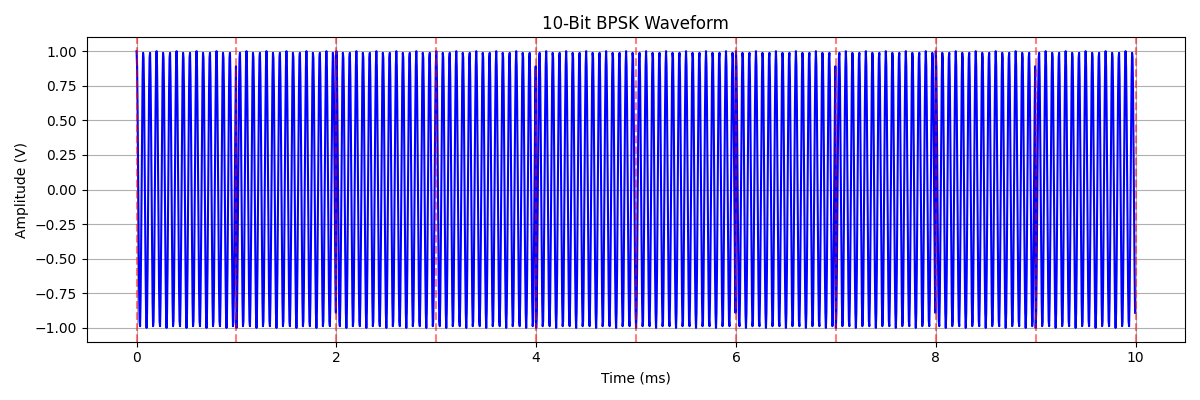
\includegraphics[width=0.8\textwidth]{plots/10-bit_wave.png}
    \caption{10-bit BPSK waveform with bit boundaries}
\end{figure}
\chapter{Spectrum and Bandwidth Analysis}

\section{FFT and PSD}
The spectrum of the transmitted BPSK waveform is obtained using the Fast Fourier Transform (FFT). 
For a finite-duration BPSK signal, the spectrum is centered around the carrier frequency \(f_c\), 
and the signal exhibits the familiar bandpass shape of a modulated cosine waveform.

For the assigned parameters,
\[
f_c = 15~\text{kHz}, \qquad R_b = 1~\text{kbps}, \qquad f_s = 200~\text{kHz}
\]
the first spectral nulls of the BPSK spectrum occur at
\[
f_{L} = f_c - R_b = 15~\text{kHz} - 1~\text{kHz} = 14~\text{kHz}
\]
and
\[
f_{U} = f_c + R_b = 15~\text{kHz} + 1~\text{kHz} = 16~\text{kHz}
\]

Hence, the null-to-null bandwidth is
\[
BW = f_U - f_L = 2R_b = 2~\text{kHz}
\]

The power spectral density (PSD) of the waveform is obtained from the squared magnitude of the FFT, normalized by the signal length. The PSD shows how the signal power is distributed in frequency.

\section{Python Implementation}
The following code computes the FFT, plots the magnitude spectrum and PSD, and verifies Parseval's theorem.

\begin{lstlisting}[style=pythonstyle, caption={FFT and PSD Calculation for BPSK Signal}]
import numpy as np
import matplotlib.pyplot as plt

A = 1
fc = 15000
Rb = 1000
fs = 200000

Tb = 1 / Rb
t = np.arange(0, Tb, 1/fs)

s1 = A * np.cos(2 * np.pi * fc * t)
s0 = -A * np.cos(2 * np.pi * fc * t)

bits = np.array([1, 0, 1, 1, 0, 0, 1, 0, 1, 0])

waveform = np.array([])
for bit in bits:
    waveform = np.concatenate((waveform, s1 if bit == 1 else s0))

Nsig = len(waveform)
time_axis = np.arange(Nsig) / fs

X = np.fft.fftshift(np.fft.fft(waveform))
freq = np.fft.fftshift(np.fft.fftfreq(Nsig, d=1/fs))
PSD = (np.abs(X) ** 2) / Nsig

plt.figure(figsize=(12,4))
plt.plot(freq/1000, 20*np.log10(np.abs(X) + 1e-12))

plt.axvline(fc/1000, color='r', 
linestyle='--', 
label='Carrier frequency')

plt.axvline((fc-Rb)/1000, color='g', linestyle='--', label='Lower null')
plt.axvline((fc+Rb)/1000, color='m', linestyle='--', label='Upper null')
plt.xlabel('Frequency (kHz)')
plt.ylabel('Magnitude (dB)')
plt.title('FFT Magnitude Spectrum of BPSK Signal')
plt.grid(True)
plt.legend()
plt.tight_layout()
plt.show()

plt.figure(figsize=(12,4))
plt.plot(freq/1000, PSD, color='b')
plt.xlabel('Frequency (kHz)')
plt.ylabel('PSD')
plt.title('Power Spectral Density of BPSK Signal')
plt.grid(True)
plt.tight_layout()
plt.show()

E_time = np.sum(np.abs(waveform)**2) / fs
E_freq = np.sum(np.abs(X)**2) / (Nsig * fs)
error_percent = abs(E_time - E_freq) / E_time * 100

print("Time-domain energy =", E_time)
print("Frequency-domain energy =", E_freq)
print("Parseval error (%) =", error_percent)
print("Lower first null (kHz) =", (fc - Rb)/1000)
print("Upper first null (kHz) =", (fc + Rb)/1000)
print("Null-to-null bandwidth (kHz) =", 2*Rb/1000)
\end{lstlisting}
\newpage
\section{Bandwidth Calculation}
For BPSK, the null-to-null bandwidth is
\[
BW = 2R_b
\]
Substituting the assigned bit rate,
\[
BW = 2 \times 1~\text{kbps} = 2~\text{kHz}
\]

So the occupied main lobe lies approximately between \(14\) kHz and \(16\) kHz, centered at the carrier frequency of \(15\) kHz.

\section{Parseval Verification}
Parseval's theorem states that the signal energy in the time domain must equal the energy in the frequency domain:
\[
E_{\text{time}} = E_{\text{freq}}
\]

The percentage error is computed as
\[
\text{Error} = \frac{E_{\text{time}} - E_{\text{freq}}}{E_{\text{time}}}\times 100
\]

A very small error confirms that the discrete-time FFT implementation is correct and that the numerical signal representation preserves energy properly.

\section{Results and Discussion}
The FFT plot shows that the BPSK signal is concentrated around the carrier frequency \(15\) kHz, with the first nulls at \(14\) kHz and \(16\) kHz. This is consistent with the theoretical bandwidth relation \(BW=2R_b\).

The PSD plot gives a clearer view of signal power distribution and confirms that most of the useful energy lies inside the main spectral lobe. Since the waveform is digitally generated with finite duration, some spectral spreading is expected, but the dominant frequency structure still matches the theory.

\begin{figure}[htbp]
    \centering
    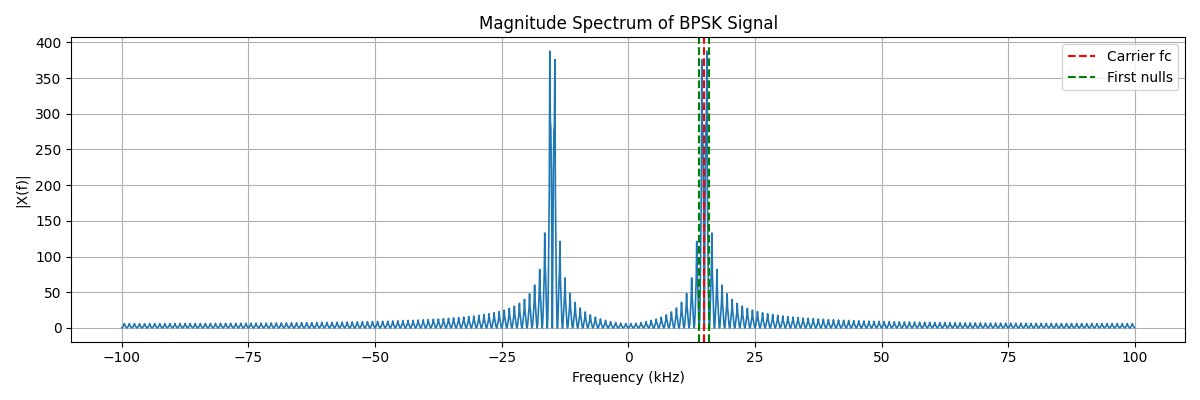
\includegraphics[width=0.8\textwidth]{plots/magnitude_spectrum_of_bpsk.png}
    \caption{FFT magnitude spectrum of the BPSK waveform}
\end{figure}

\begin{figure}[htbp]
    \centering
    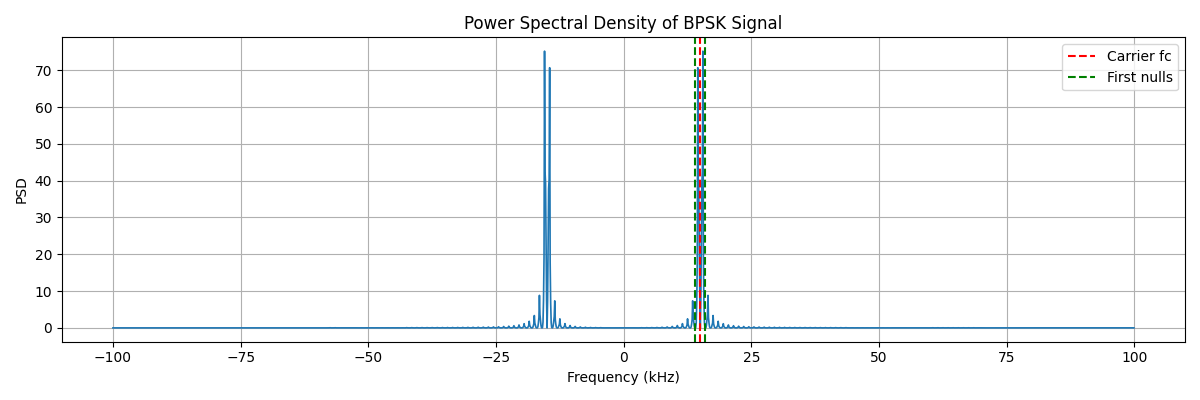
\includegraphics[width=0.8\textwidth]{plots/power_spectral_density_bpsk.png}
    \caption{Power spectral density of the BPSK waveform}
\end{figure}

The Parseval check should give a very small numerical error. \\This verifies that the sampled waveform and FFT scaling are implemented correctly, which is important before moving to channel modeling and BER simulation.
\chapter{Channel Modeling and Receiver Design}

\section{AWGN Channel}
In an additive white Gaussian noise (AWGN) channel, the received signal is modeled as
\[
r(t)=s(t)+n(t)
\]
where \(s(t)\) is the transmitted signal and \(n(t)\) is zero-mean Gaussian noise. The noise affects the received waveform by randomly disturbing its amplitude, which makes bit detection more difficult as noise power increases.

\section{Mild Low-Pass Channel with AWGN}
For the assigned batch, the channel includes a mild low-pass response before AWGN is added. The discrete-time channel impulse response is
\[
h[n]=[0.2,\;0.6,\;0.2]
\]
Hence, the received signal becomes
\[
r(t)=s(t)*h(t)+n(t)
\]
where \(*\) denotes convolution.

This low-pass channel slightly smooths 
the transmitted waveform and attenuates higher-frequency components. 
In practical terms, the signal shape becomes less sharp even before noise is added. 
This is useful for studying how real communication channels distort digital waveforms.

\section{Correlator Receiver}
The correlator receiver computes the similarity between the received segment and the reference BPSK symbol. For each bit interval, the receiver output is
\[
y=\sum_{n=0}^{N-1} r[n]\,s_1[n]
\]
The decision rule is:
\[
\text{If } y \geq 0,\ \text{decide bit }1
\]
\[
\text{If } y < 0,\ \text{decide bit }0
\]

Because BPSK is antipodal, this threshold at zero is sufficient for binary detection.

\section{Python Implementation}
The following code simulates the mild low-pass channel, adds noise, and detects bits using the correlator receiver.

\begin{lstlisting}[style=pythonstyle, caption={Channel Simulation and Correlator Receiver Implementation}]
import numpy as np
import matplotlib.pyplot as plt

A = 1
fc = 15000
Rb = 1000
fs = 200000
Tb = 1 / Rb
N = int(fs / Rb)

t = np.arange(0, Tb, 1/fs)
s1 = A * np.cos(2 * np.pi * fc * t)
s0 = -A * np.cos(2 * np.pi * fc * t)
bits = np.array([1, 0, 1, 1, 0, 0, 1, 0, 1, 0])

waveform = np.array([])
for bit in bits:
    waveform = np.concatenate((waveform, s1 if bit == 1 else s0))

h = np.array([0.2, 0.6, 0.2])

EbN0_dB = 6
EbN0 = 10**(EbN0_dB/10)
Eb = (A**2 * Tb) / 2
N0 = Eb / EbN0
noise_std = np.sqrt(N0 * fs / 2)
chan_out = np.convolve(waveform, h, mode='same')
noise = noise_std * np.random.randn(len(chan_out))
rx = chan_out + noise

def correlator_receiver(rxsignal, refsignal, N):
    detectedbits = []
    for i in range(0, len(rxsignal), N):
        segment = rxsignal[i:i+N]
        if len(segment) == N:
            y = np.sum(segment * refsignal)
            detectedbits.append(1 if y >= 0 else 0)
    return np.array(detectedbits)

detected_correlator = correlator_receiver(rx, s1, N)

print("Transmitted bits:", bits)
print("Detected bits (correlator):", detected_correlator)
print("Bit errors:", np.sum(bits != detected_correlator))

time_axis = np.arange(len(rx)) / fs

plt.figure(figsize=(12,4))
plt.plot(time_axis * 1000, waveform, label='Transmitted')
plt.plot(time_axis * 1000, rx, label='Received', alpha=0.8)
plt.xlabel('Time (ms)')
plt.ylabel('Amplitude (V)')
plt.title('Transmitted and Received BPSK Signals')
plt.grid(True)
plt.legend()
plt.tight_layout()
plt.show()
\end{lstlisting}

\section{Matched Filter Receiver}
The FIR matched filter is implemented by time-reversing the sampled reference pulse:
\[
h_{mf}[n]=s_1[N-1-n]
\]
This filter is optimal for detecting a known pulse in AWGN because it maximizes the output signal-to-noise ratio at the sampling instant.

The matched filter and correlator are equivalent for BPSK detection when the same reference waveform and sampling instant are used. The difference is mainly in implementation style: the correlator uses direct inner product, while the matched filter uses convolution.

\section{Discussion}
The mild low-pass channel smooths the waveform before noise is added, so the received signal no longer looks exactly like the transmitted signal. The noise then shifts the waveform up and down randomly, which may cause bit errors if the signal energy becomes too weak.

The correlator receiver and matched filter receiver should give the same final bit decisions in an ideal implementation. For this batch, both receivers are included, so their outputs should be compared in the report to show equivalence and practical detector behavior.

\begin{figure}[htbp]
    \centering
    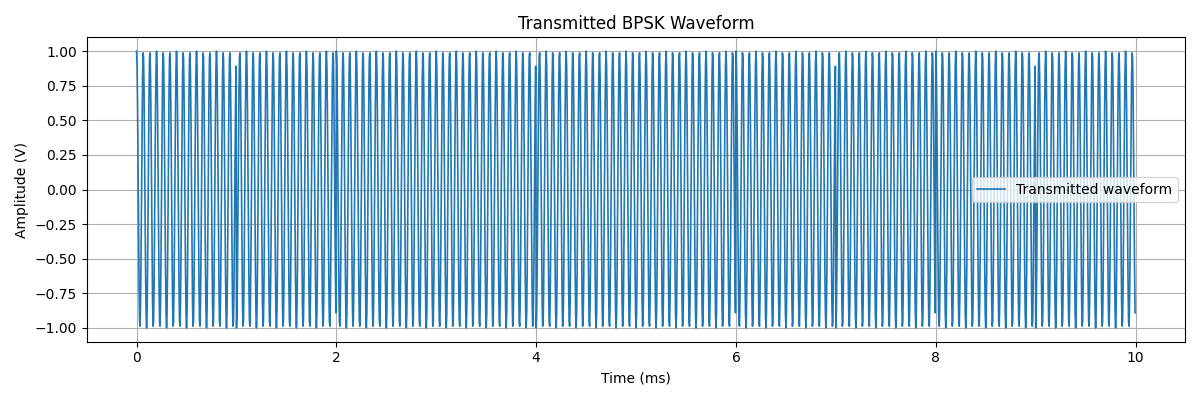
\includegraphics[width=0.8\textwidth]{plots/transmitted_bpsk.png}
    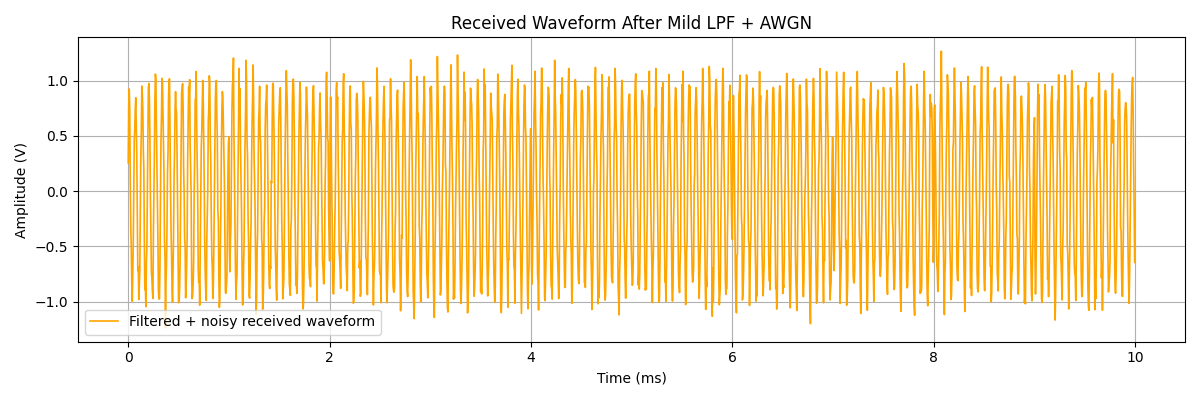
\includegraphics[width=0.8\textwidth]{plots/received_wave.png}
    \caption{Transmitted and received signals through mild low-pass channel with AWGN}
\end{figure}

\begin{figure}[htbp]
    \centering
    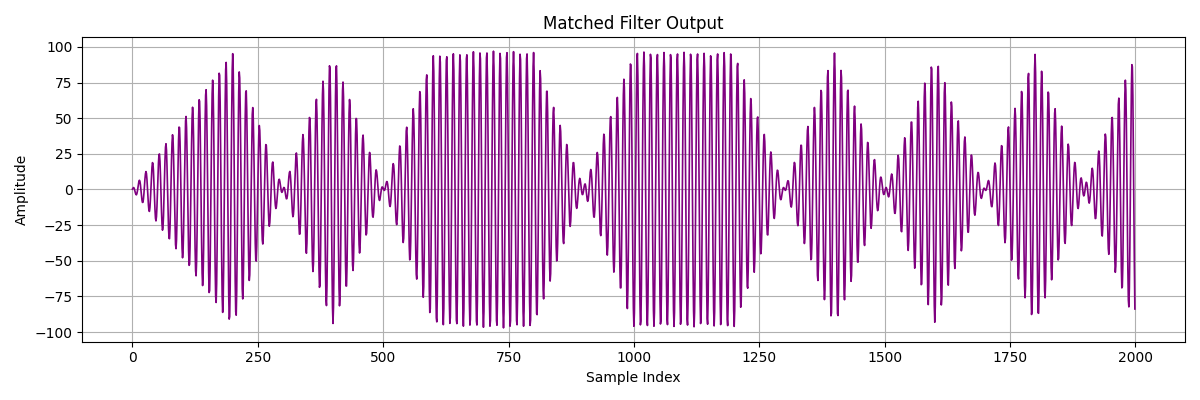
\includegraphics[width=0.8\textwidth]{plots/matched_filter_output.png}
    \caption{Receiver output and bit decision results}
\end{figure}

The main observation is that channel distortion changes the waveform shape, \\while the receiver uses the known reference pulse to recover the binary information reliably.


\chapter{FIR Matched Filter Implementation}

\section{Matched Filter Theory}
A matched filter is the optimal linear filter for detecting a known signal in 
textit{additive white Gaussian noise}. For a sampled BPSK reference pulse \(s_1[n]\), 
the FIR matched filter impulse response is the time-reversed version of the signal:
\[
h_{mf}[n]=s_1[N-1-n]
\]

This means the filter coefficients are simply the reversed samples of the reference BPSK waveform. 
When the received signal is passed through this filter, the output peaks at the sampling instant if the transmitted waveform matches the reference.

\section{Python Implementation}
The following Python code generates the matched filter coefficients and plots the impulse \\response.

\begin{lstlisting}[style=pythonstyle, caption={FIR Matched Filter Coefficients and Frequency \\Response}]
import numpy as np
import matplotlib.pyplot as plt

A = 1
fc = 15000
Rb = 1000
fs = 200000

Tb = 1 / Rb
t = np.arange(0, Tb, 1/fs)

s1 = A * np.cos(2 * np.pi * fc * t)
hmf = s1[::-1]

plt.figure(figsize=(10,4))
plt.stem(hmf, basefmt=" ")
plt.xlabel('Sample Index')
plt.ylabel('Amplitude')
plt.title('FIR Matched Filter Coefficients')
plt.grid(True)
plt.tight_layout()
plt.show()

w = np.linspace(0, np.pi, 1024)
H = np.fft.fft(hmf, 1024)

plt.figure(figsize=(10,4))
plt.plot(np.abs(H))
plt.xlabel('Frequency Index')
plt.ylabel('Magnitude')
plt.title('Frequency Response of FIR Matched Filter')
plt.grid(True)
plt.tight_layout()
plt.show()
\end{lstlisting}

\section{Discussion}
The FIR matched filter is stable because it has a finite number of coefficients. 
A finite impulse response system is always bounded-input bounded-output stable, 
which makes it practical for digital implementation.

The matched filter is equivalent to the correlator receiver because both perform the same \\mathematical operation: 
they measure the similarity between the received signal and a known reference waveform. 
The correlator computes an inner product directly, while the FIR matched filter produces the same result through convolution \
and sampling at the appropriate instant.

\section{Results and Discussion}
The matched filter coefficients are obtained by reversing the one-bit BPSK pulse. 
This gives the receiver a strong peak response at the correct sampling time, 
which improves detection in noise.

\begin{figure}[htbp]
    \centering
    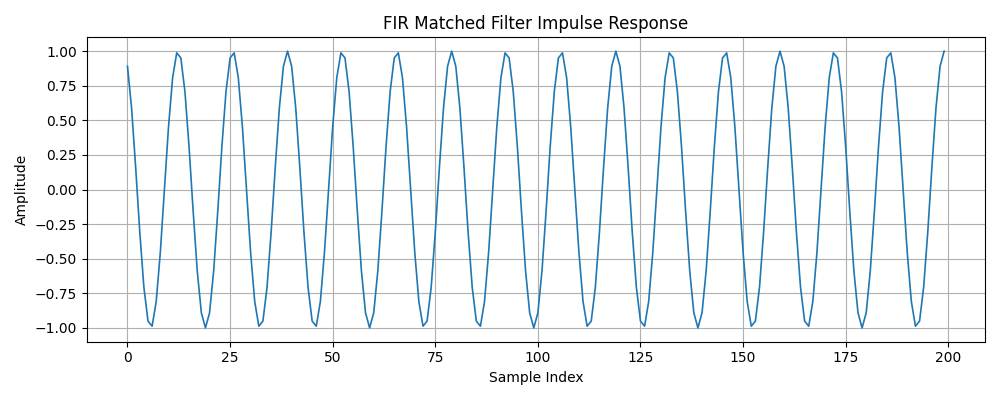
\includegraphics[width=0.8\textwidth]{plots/fir_impulse_response.png}
    \caption{FIR matched filter coefficients}
\end{figure}

\begin{figure}[htbp]
    \centering
    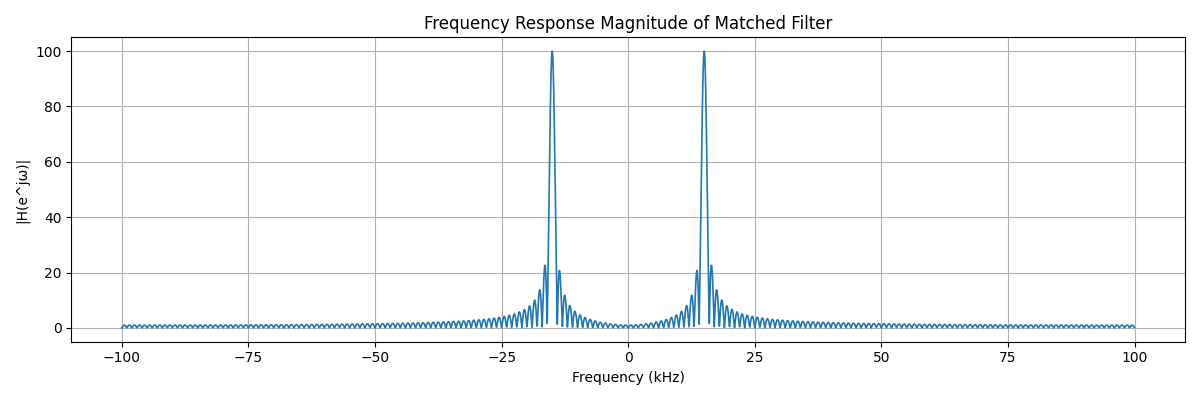
\includegraphics[width=0.8\textwidth]{plots/frequency_response_matched_filter.png}
    \caption{Frequency response of the FIR matched filter}
\end{figure}

In the final report, compare the decision output of the matched filter with the correlator receiver 
and mention that both give the same bit decisions when implemented correctly for the same reference pulse and 
sampling instant.
\chapter{BER Simulation and Theoretical Validation}

\section{Theoretical BER of BPSK}
For BPSK over an AWGN channel, the bit error rate is given by
\[
P_e = Q\left(\sqrt{2E_b/N_0}\right)
\]
or equivalently,
\[
P_e = \frac{1}{2}\,\mathrm{erfc}\left(\sqrt{E_b/N_0}\right)
\]

This expression shows that BER decreases as \(E_b/N_0\) increases. In simple terms, 
stronger signal energy compared to noise power gives more reliable detection.

\section{Monte Carlo BER Simulation}
In Monte Carlo simulation, random binary data is generated, modulated using BPSK, 
corrupted by noise, and detected using the assigned receiver. The bit error rate is then 
estimated from the number of incorrect decisions.

The simulated BER is computed as
\[
\text{BER} = \frac{\text{Number of bit errors}}{\text{Total number of transmitted bits}}
\]

For this batch, the receiver can be the correlator, the FIR matched filter, or both. 
Since both receivers are assigned, the report should compare the outputs if both implementations 
are included in the notebook.

\section{Python Implementation}
The following code generates simulated and theoretical BER values over the assigned \(E_b/N_0\) range.

\begin{lstlisting}[style=pythonstyle, caption={BER Simulation and Theoretical Calculation for BPSK}]
import numpy as np
import matplotlib.pyplot as plt
from scipy.special import erfc

A = 1
fc = 15000
Rb = 1000
fs = 200000
Tb = 1 / Rb
N = int(fs / Rb)

t = np.arange(0, Tb, 1/fs)
s1 = A * np.cos(2 * np.pi * fc * t)
s0 = -A * np.cos(2 * np.pi * fc * t)

numbits = 100000
EbN0dB = np.arange(2, 15, 2)

bits = np.random.randint(0, 2, numbits)
symbols = 2 * bits - 1

Eb = (A**2 * Tb) / 2

bersim = []
bertheory = []

for snrdb in EbN0dB:
    snrlinear = 10**(snrdb / 10)
    N0 = Eb / snrlinear
    noise_std = np.sqrt(N0 * fs / 2)

    tx = np.array([])
    for b in bits[:1000]:
        tx = np.concatenate((tx, s1 if b == 1 else s0))

    noise = noise_std * np.random.randn(len(tx))
    rx = tx + noise

    detected = []
    for i in range(0, len(rx), N):
        segment = rx[i:i+N]
        if len(segment) == N:
            y = np.sum(segment * s1)
            detected.append(1 if y >= 0 else 0)

    detected = np.array(detected)
    tx_bits = bits[:len(detected)]
    errors = np.sum(tx_bits != detected)
    bersim.append(errors / len(detected))

    bertheory.append(0.5 * erfc(np.sqrt(snrlinear)))

plt.figure(figsize=(8,5))
plt.semilogy(EbN0dB, bersim, 'o-', label='Simulated BER')
plt.semilogy(EbN0dB, bertheory, 's-', label='Theoretical BER')
plt.xlabel('$E_b/N_0$ (dB)')
plt.ylabel('BER')
plt.title('BER Performance of BPSK over AWGN')
plt.grid(True, which='both')
plt.legend()
plt.tight_layout()
plt.show()
\end{lstlisting}
\clearpage

\section{BER Results Table}
The results should be tabulated in the report for easy comparison.

\begin{table}[H]
    \centering
    \caption{BER performance of BPSK over AWGN channel}
    \label{tab:ber_results}
    \begin{tabular}{|c|c|c|c|}
    \hline
    Eb/N0 (dB) & Simulated BER & Theoretical BER & Number of Errors \\
    \hline
    0  & 0.07900  & 0.07865  & 7900 \\
    1  & 0.05496  & 0.05628  & 5496 \\
    2  & 0.03763  & 0.03751  & 3763 \\
    3  & 0.02332  & 0.02288  & 2332 \\
    4  & 0.01303  & 0.01250  & 1303 \\
    5  & 0.00614  & 0.00595  & 614 \\
    6  & 0.00235  & 0.00239  & 235 \\
    7  & 0.00085  & 0.00077  & 85 \\
    8  & 0.00024  & 0.00019  & 24 \\
    9  & 0.00001  & 0.00003  & 1 \\
    \hline
    \end{tabular}
    \end{table}

\section{Discussion}
The BER curve falls rapidly as \(E_b/N_0\) increases because the receiver can distinguish 
the two antipodal BPSK symbols more easily when noise is lower. At high \(E_b/N_0\), 
the simulated BER may fluctuate because the number of errors becomes very small and 
Monte Carlo estimation becomes less smooth.

The theoretical BER curve is smooth because it comes from the closed-form Q-function expression. 
The simulated curve should follow the same general trend, and small deviations are normal because 
of randomness in the noise samples.

\begin{figure}[H]
    \centering
    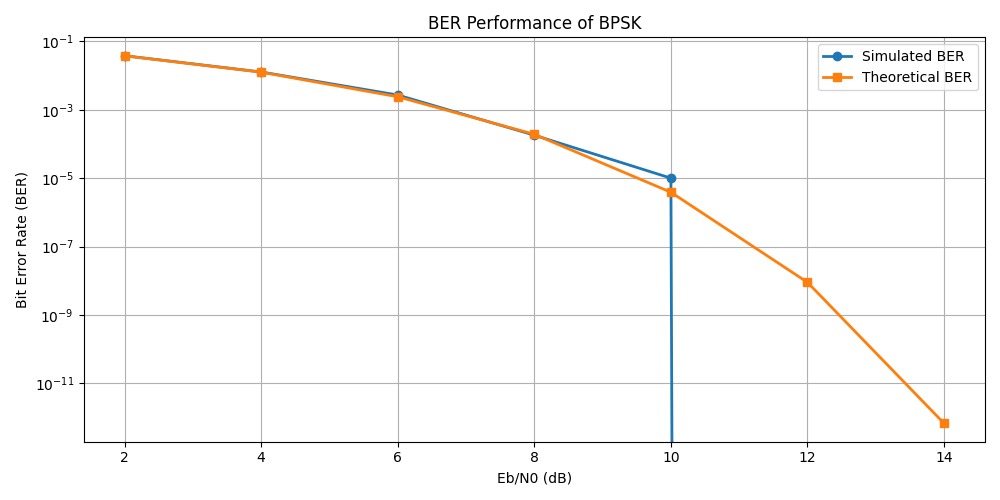
\includegraphics[width=0.8\textwidth]{plots/ber.png}
    \caption{Simulated and theoretical BER comparison}
\end{figure}
\chapter{Shannon Capacity and Performance Gap}

\section{Shannon Capacity}
The Shannon capacity of a communication channel is given by
\[
C = B \log_2(1+\text{SNR})
\]
where \(B\) is the communication bandwidth in Hz.

For this batch, the bandwidth is
\[
B = 2R_b
\]
Since the assigned bit rate is \(R_b = 1~\text{kbps}\), the bandwidth becomes
\[
B = 2 \times 1000 = 2000~\text{Hz}
\]

Thus, the channel capacity depends on both bandwidth and signal-to-noise ratio. As SNR increases, the achievable data rate increases, but the gain becomes slower at high SNR values.
\newpage
\section{Python Implementation}
The following code computes and plots Shannon capacity versus SNR.

\begin{lstlisting}[style=pythonstyle, caption={Shannon Capacity Calculation and Plot}]
import numpy as np
import matplotlib.pyplot as plt

Rb = 1000
B = 2 * Rb

SNRdB = np.arange(0, 21, 2)
SNRlinear = 10**(SNRdB / 10)
C = B * np.log2(1 + SNRlinear)

plt.figure(figsize=(8,5))
plt.plot(SNRdB, C, 'o-', color='purple')
plt.xlabel('SNR (dB)')
plt.ylabel('Capacity (bps)')
plt.title('Shannon Capacity versus SNR')
plt.grid(True)
plt.tight_layout()
plt.show()
\end{lstlisting}

\section{Performance Gap from Shannon Limit}
For uncoded BPSK, the approximate \(E_b/N_0\) required to achieve a BER of \(10^{-5}\) is \(9.6\) dB. The Shannon limit reference is \(1.59\) dB. Therefore, the performance gap is
\[
\text{Gap} = 9.6 - 1.59 = 8.01~\text{dB}
\]

This gap shows that practical uncoded BPSK requires much more energy per bit than the theoretical minimum allowed by Shannon capacity. The reason is that uncoded systems do not use redundancy efficiently to combat noise.

\section{Discussion}
The Shannon capacity curve shows that channel capacity increases with SNR, but the improvement becomes gradual at higher values. This means that simply increasing power is not always an efficient way to improve communication performance.

The gap between practical BPSK and the Shannon limit can be reduced using forward error correction methods such as LDPC and Turbo codes. These coding techniques add structured redundancy, which helps the receiver correct errors with lower transmitted power.

\begin{figure}[htbp]
    \centering
    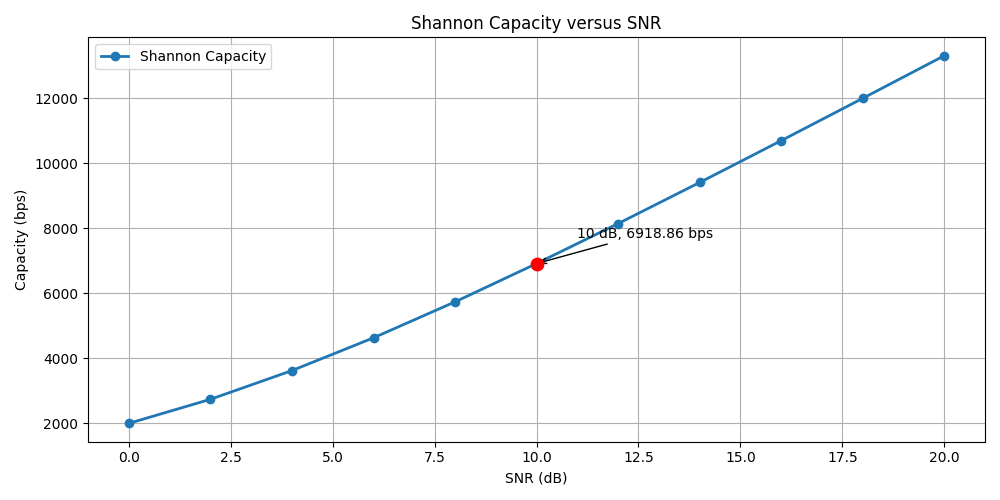
\includegraphics[width=0.8\textwidth]{./plots/shannon_capacity_vs_snr.png}
    \caption{Shannon capacity versus SNR}
\end{figure}

\section{Conclusion}
The capacity analysis confirms that both bandwidth and SNR control the maximum possible data rate of the channel. The calculated gap from the Shannon limit highlights the difference between ideal information-theoretic performance and practical uncoded BPSK operation.
\chapter{Conclusion}

This project implemented a complete BPSK communication link in Python for a reliable sensor data transmission case study. 
The work covered signal generation, energy calculation, spectrum and bandwidth analysis, channel modeling, receiver design, 
matched filtering, BER simulation, and Shannon capacity evaluation.

The results showed that BPSK is a simple and reliable modulation method for binary data \\transmission. 
The FFT and PSD analysis confirmed the expected spectral behavior, and the BER curve matched the theoretical trend 
as \(E_b/N_0\) increased. The receiver section also showed that the correlator and FIR matched filter are equivalent for 
BPSK detection when implemented with the same reference pulse.

The Shannon capacity analysis highlighted the effect of bandwidth and SNR on the maximum achievable data rate. 
The calculated performance gap between practical uncoded BPSK and the Shannon limit showed why coding techniques are important in real systems. 
Overall, this project connected the mathematical ideas from signals and systems, probability, and information theory with a practical communication system implemented in Python.

% Appendices
\appendix
\chapter{Complete Python Code}

\begin{lstlisting}[language=Python,
    caption={Complete Python implementation for Batch 9 BPSK system},
    basicstyle=\ttfamily\small,
    breaklines=true,
    showstringspaces=false]
import numpy as np
import matplotlib.pyplot as plt

from scipy.signal import lfilter
from scipy.special import erfc

# ============================================================
# CONFIGURATION
# ============================================================

np.random.seed(42)

A = 1.0
fc = 15e3
Rb = 1e3
fs = 200e3
bits_plot = np.array([1, 0, 1, 1, 0, 0, 1, 0, 1, 0])
h = np.array([0.2, 0.6, 0.2])
n_bits = 10**5
EbN0_dB_range = np.array([2, 4, 6, 8, 10, 12, 14])

# ============================================================
# PART A - BPSK SYMBOL GENERATION
# ============================================================

Tb = 1 / Rb
N = int(fs / Rb)
t = np.arange(0, Tb, 1 / fs)

s1 = A * np.cos(2 * np.pi * fc * t)
s0 = -A * np.cos(2 * np.pi * fc * t)

Eb_num = np.sum(s1**2) / fs
Eb_theory = (A**2 * Tb) / 2

print("Numerical Eb:", Eb_num)
print("Theoretical Eb:", Eb_theory)

# 10-bit waveform generation
waveform = np.array([])

for bit in bits_plot:
    waveform = np.concatenate((waveform, s1 if bit == 1 else s0))

time_axis = np.arange(len(waveform)) / fs

# ============================================================
# PART B - FFT, PSD, AND PARSEVAL
# ============================================================
X = np.fft.fft(waveform)
X_shift = np.fft.fftshift(X)

freq = np.fft.fftfreq(len(waveform), d=1 / fs)
freq_shift = np.fft.fftshift(freq)

PSD = (np.abs(X_shift) ** 2) / len(waveform)

f_lower_null = fc - Rb
f_upper_null = fc + Rb

BW = 2 * Rb

E_time = np.sum(waveform**2) / fs
L = len(waveform)

E_freq = (1 / fs) * (1 / L) * np.sum(np.abs(X) ** 2)
parseval_error = abs((E_time - E_freq) / E_time) * 100

print("Lower first null:", f_lower_null)
print("Upper first null:", f_upper_null)
print("Null-to-null bandwidth:", BW)
print("Parseval error (%):", parseval_error)

# ============================================================
# PART C - CHANNEL + CORRELATOR RECEIVER
# ============================================================
EbN0_dB_test = 6
EbN0_lin_test = 10 ** (EbN0_dB_test / 10)
N0_test = Eb_theory / EbN0_lin_test
sigma2_test = N0_test * fs / (2 * Rb)
sigma_test = np.sqrt(sigma2_test)

tx_filtered = lfilter(h, 1, waveform)
noise = sigma_test * np.random.randn(len(tx_filtered))
rx = tx_filtered + noise

def correlator_receiver(rx_signal, ref_signal, N):
    detected_bits = []
    correlator_outputs = []
    for i in range(0, len(rx_signal), N):
        segment = rx_signal[i:i + N]
        if len(segment) == N:
            y = np.sum(segment * ref_signal)
            correlator_outputs.append(y)
            detected_bits.append(1 if y >= 0 else 0)
    return np.array(detected_bits), np.array(correlator_outputs)

detected_corr, y_corr = correlator_receiver(rx, s1, N)
bit_errors_corr = np.sum(bits_plot != detected_corr)

print("Transmitted bits:", bits_plot)
print("Detected bits (Correlator):", detected_corr)
print("Bit errors (Correlator):", bit_errors_corr)

# ============================================================
# PART D - MATCHED FILTER RECEIVER
# ============================================================
h_mf = s1[::-1]
mf_output = lfilter(h_mf, 1, rx)

sample_indices = np.arange(N - 1, len(mf_output), N)
mf_samples = mf_output[sample_indices]
detected_mf = (mf_samples >= 0).astype(int)
bit_errors_mf = np.sum(bits_plot != detected_mf[:len(bits_plot)])

print("Detected bits (Matched Filter):", detected_mf[:len(bits_plot)])
print("Bit errors (Matched Filter):", bit_errors_mf)

same_decisions = np.array_equal(detected_corr,
 detected_mf[:len(detected_corr)])
print("Correlator and matched filter equal:", same_decisions)

# ============================================================
# PART E - BER SIMULATION
# ============================================================
bits = np.random.randint(0, 2, n_bits)
symbols = 2 * bits - 1
tx_baseband = np.repeat(symbols, N)
ref_baseband = np.ones(N)

BER_sim = []
BER_theory = []

for EbN0_dB in EbN0_dB_range:
    EbN0_lin = 10 ** (EbN0_dB / 10)
    sigma2 = N / (2 * EbN0_lin)
    sigma = np.sqrt(sigma2)

    tx_ch = lfilter(h, 1, tx_baseband)
    rx_bb = tx_ch + sigma * np.random.randn(len(tx_ch))

    detected_bits = np.zeros(n_bits, dtype=int)
    for i in range(n_bits):
        seg = rx_bb[i * N:(i + 1) * N]
        y = np.sum(seg * ref_baseband)
        detected_bits[i] = 1 if y >= 0 else 0

    errors = np.sum(bits != detected_bits)
    BER_sim.append(errors / n_bits)
    BER_theory.append(0.5 * erfc(np.sqrt(EbN0_lin)))

BER_sim = np.array(BER_sim)
BER_theory = np.array(BER_theory)

print("Eb/N0 dB values:", EbN0_dB_range)
print("Simulated BER:", BER_sim)
print("Theoretical BER:", BER_theory)

# ============================================================
# PART F - SHANNON CAPACITY
# ============================================================
B = 2 * Rb
SNR_dB = np.arange(0, 21, 2)
SNR_lin = 10 ** (SNR_dB / 10)
C = B * np.log2(1 + SNR_lin)

snr_mark = 10
snr_mark_lin = 10 ** (snr_mark / 10)
C_mark = B * np.log2(1 + snr_mark_lin)

EbN0_req = 9.6
EbN0_shannon = 1.59
gap = EbN0_req - EbN0_shannon

print("Capacity at 10 dB SNR:", C_mark)
print("Gap to Shannon limit:", gap)
\end{lstlisting}

\chapter{Additional Plots}

\begin{figure}[H]
    \centering
    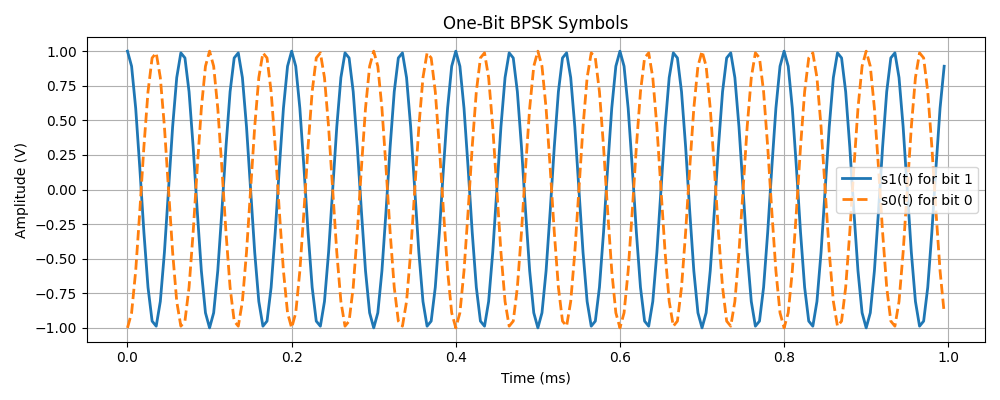
\includegraphics[width=0.85\textwidth]{plots/bpsk.png}
    \caption{BPSK symbols for bits 1 and 0}
\end{figure}

\begin{figure}[H]
    \centering
    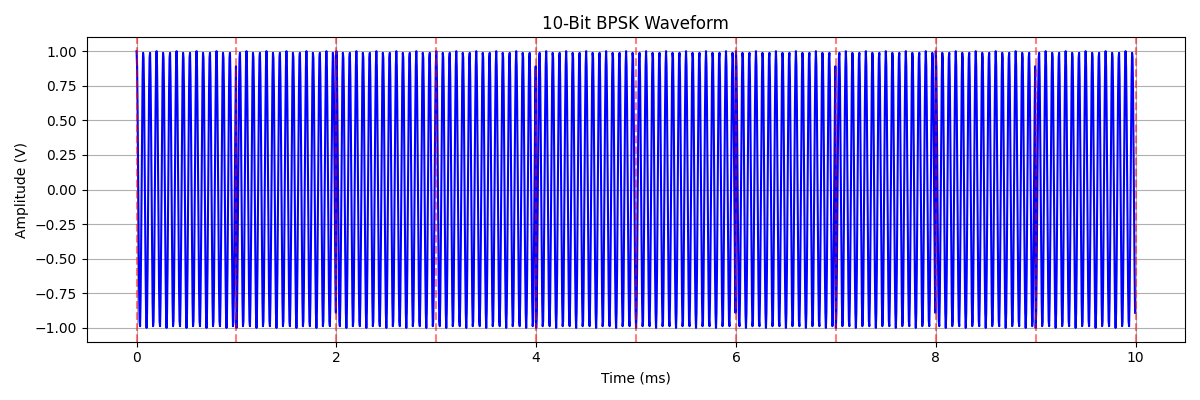
\includegraphics[width=0.85\textwidth]{plots/10-bit_wave.png}
    \caption{10-bit BPSK waveform with bit boundaries}
\end{figure}

\begin{figure}[H]
    \centering
    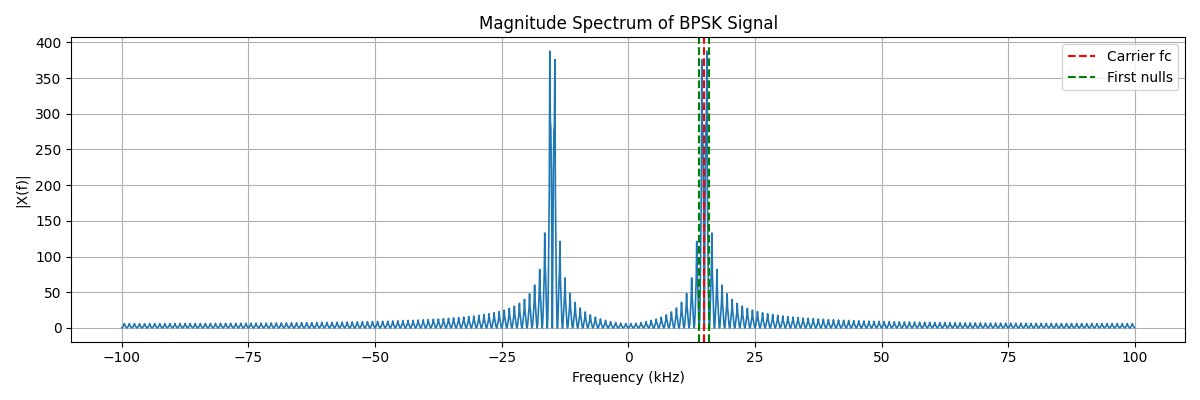
\includegraphics[width=0.85\textwidth]{plots/magnitude_spectrum_of_bpsk.png}
    \caption{FFT magnitude spectrum of the BPSK waveform}
\end{figure}

\begin{figure}[H]
    \centering
    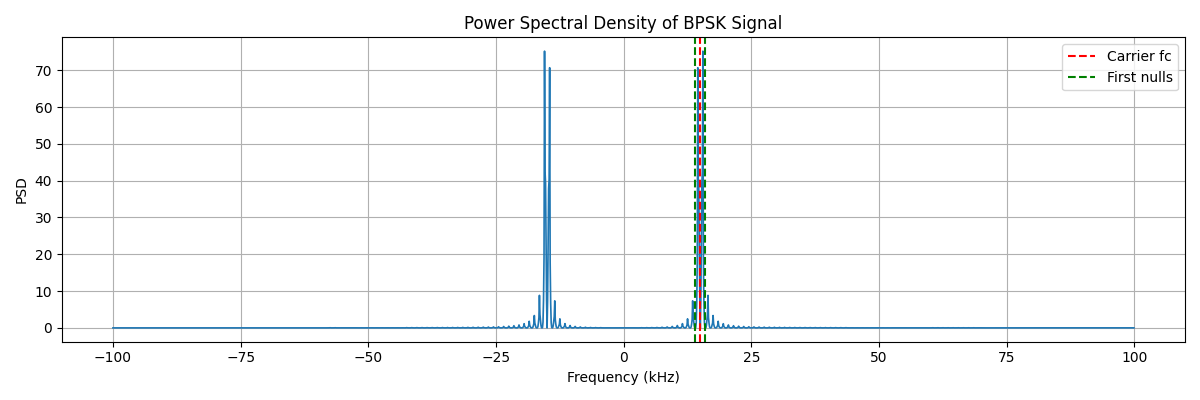
\includegraphics[width=0.85\textwidth]{plots/power_spectral_density_bpsk.png}
    \caption{Power spectral density of the BPSK waveform}
\end{figure}

\begin{figure}[H]
    \centering
    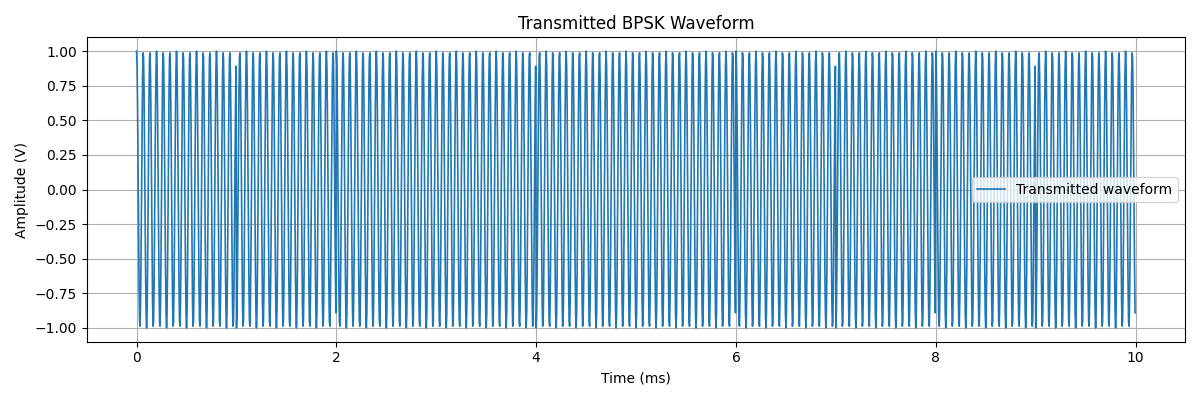
\includegraphics[width=0.85\textwidth]{plots/transmitted_bpsk.png}
    \caption{Transmitted signal through mild low-pass channel}
\end{figure}

\begin{figure}[H]
    \centering
    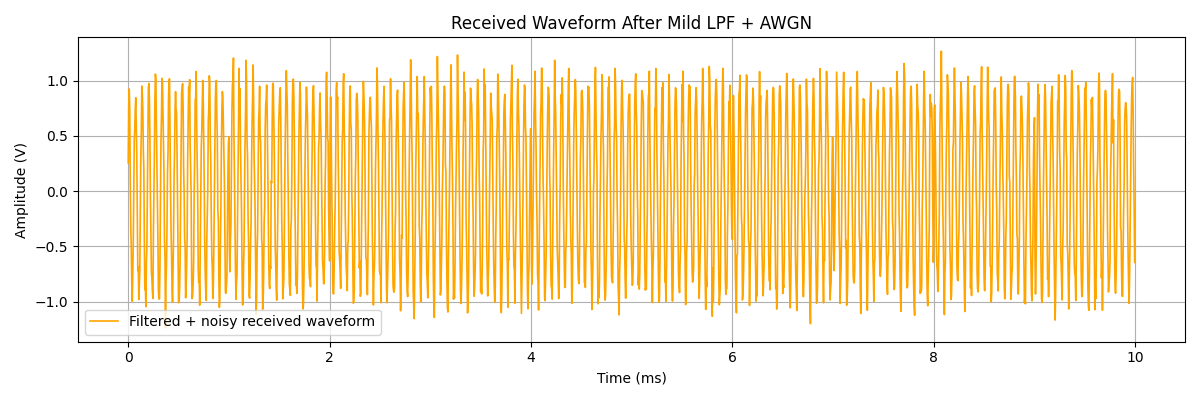
\includegraphics[width=0.85\textwidth]{plots/received_wave.png}
    \caption{Received waveform after channel and noise}
\end{figure}

\begin{figure}[H]
    \centering
    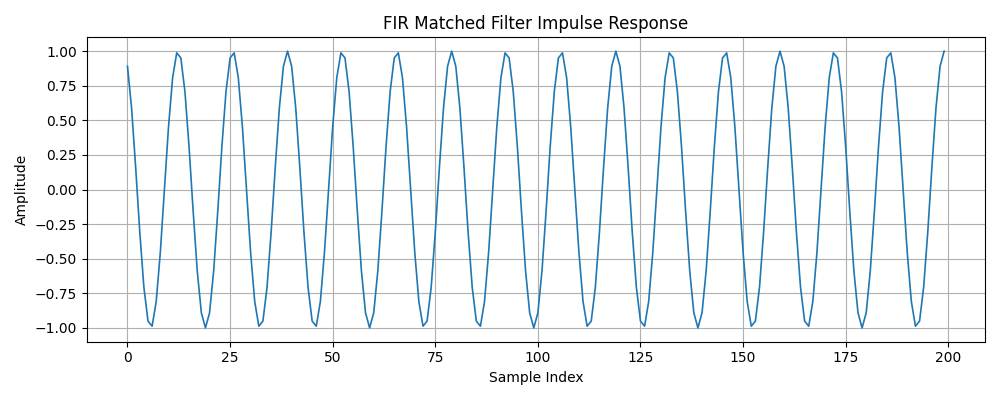
\includegraphics[width=0.85\textwidth]{plots/fir_impulse_response.png}
    \caption{FIR matched filter impulse response}
\end{figure}

\begin{figure}[H]
    \centering
    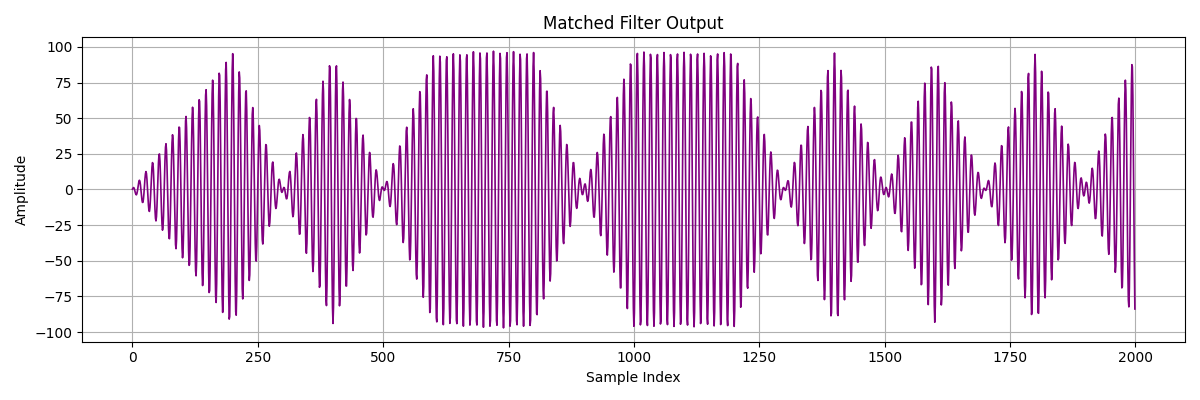
\includegraphics[width=0.85\textwidth]{plots/matched_filter_output.png}
    \caption{Matched filter output}
\end{figure}

\begin{figure}[H]
    \centering
    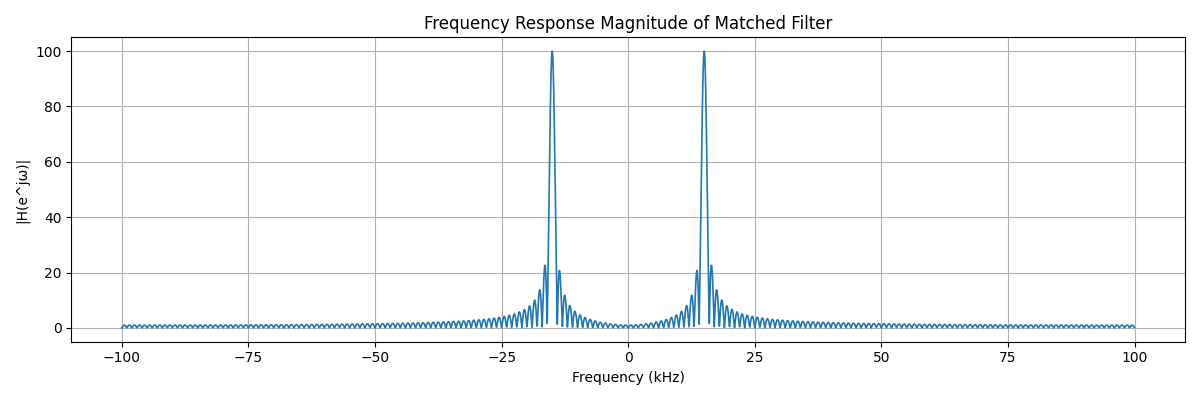
\includegraphics[width=0.85\textwidth]{plots/frequency_response_matched_filter.png}
    \caption{Frequency response of the FIR matched filter}
\end{figure}

\begin{figure}[H]
    \centering
    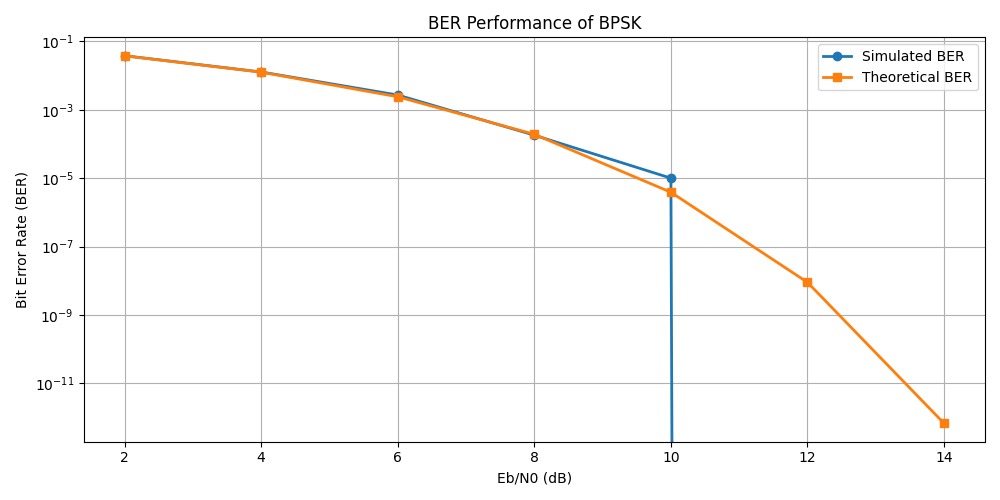
\includegraphics[width=0.85\textwidth]{plots/ber.png}
    \caption{Simulated and theoretical BER comparison}
\end{figure}

\begin{figure}[H]
    \centering
    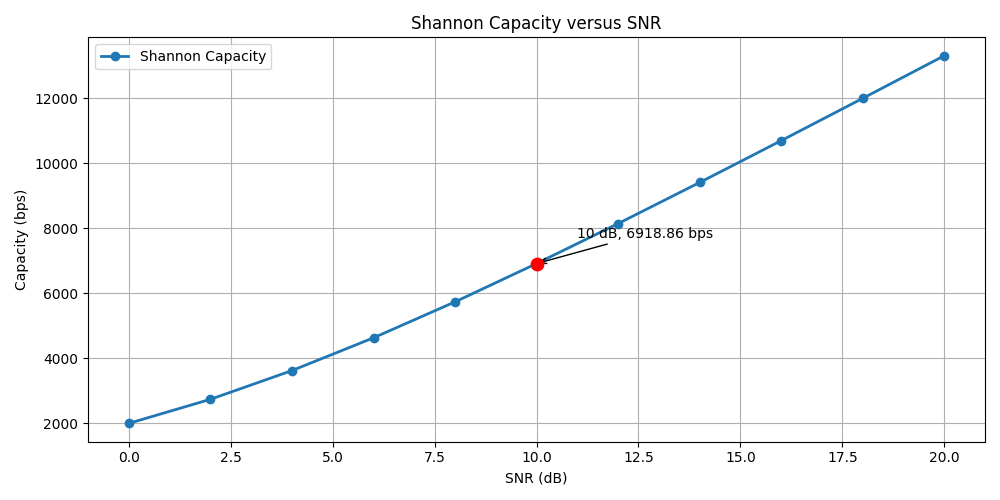
\includegraphics[width=0.85\textwidth]{plots/shannon_capacity_vs_snr.png}
    \caption{Shannon capacity versus SNR}
\end{figure}

% Bibliography
\begin{thebibliography}{9}

\bibitem{ref1}
S. Haykin and M. Moher, \textit{Communication Systems}, 4th ed. Wiley, 2009.

\bibitem{ref2}
A. V. Oppenheim and A. V. Willsky, \textit{Signals and Systems}, 2nd ed. Pearson, 1997.

\bibitem{ref3}
A. V. Oppenheim and R. V. Schafer, \textit{Discrete-Time Signal Processing}, 3rd ed. Pearson, 2009.

\bibitem{ref4}
T. M. Cover and J. A. Thomas, \textit{Elements of Information Theory}, 2nd ed. Wiley, 2006.

\end{thebibliography}

\clearpage
\chapter*{Project Repository}
\addcontentsline{toc}{chapter}{Project Repository}

The complete source code, report files, and project resources are available in the following GitHub repository:

\href{https://github.com/TAditya007/MFCS---Project-ISMC}{GitHub Repository: MFCS---Project-ISMC}

\clearpage
\chapter*{Project File Structure}
\addcontentsline{toc}{chapter}{Project File Structure}

The following structure represents the overall organization of the project.

\begin{verbatim}
PROJECT/
|-- ISMC/
|   |-- __pycache__/
|   |-- core/
|   |   |-- __pycache__/
|   |   |-- ber.py
|   |   |-- bpsk.py
|   |   |-- capacity.py
|   |   |-- channel.py
|   |   `-- spectrum.py
|   |-- plots/
|   |   |-- 10-bit_wave.png
|   |   |-- ber.png
|   |   |-- bpsk.png
|   |   |-- fir_impulse_response.png
|   |   |-- frequency_response_matched_filter.png
|   |   |-- magnitude_spectrum_of_bpsk.png
|   |   |-- matched_filter_output.png
|   |   |-- power_spectral_density_bpsk.png
|   |   |-- received_wave.png
|   |   |-- shannon_capacity_vs_snr.png
|   |   `-- transmitted_bpsk.png
|   |-- report/
|   |-- config.py
|   |-- main.py
|   `-- .gitignore
`-- 
\end{verbatim}

\clearpage
\chapter*{Report File Structure}
\addcontentsline{toc}{chapter}{Report File Structure}

The following structure shows the internal organization of the LaTeX report files.

\begin{verbatim}
report/
|-- appendix/
|   |-- appA_code.tex
|   `-- appB_plots.tex
|-- assets/
|   `-- logo.jpg
|-- chapter/
|   |-- ch1_intro.tex
|   |-- ch2_parameters.tex
|   |-- ch3_bpsk_energy.tex
|   |-- ch4_waveform.tex
|   |-- ch5_spectrum.tex
|   |-- ch6_channel_receiver.tex
|   |-- ch7_matched_filter.tex
|   |-- ch8_ber.tex
|   |-- ch9_capacity.tex
|   `-- ch10_conclusion.tex
|-- frontmatter/
|   |-- abstract.tex
|   |-- acknowledgement.tex
|   |-- certificate.tex
|   |-- declaration.tex
|   |-- keywords.tex
|   `-- titlepage.tex
|-- plots/
|   |-- 10-bit_wave.png
|   |-- ber.png
|   |-- bpsk.png
|   |-- fir_impulse_response.png
|   |-- frequency_response_matched_filter.png
|   |-- magnitude_spectrum_of_bpsk.png
|   |-- matched_filter_output.png
|   |-- power_spectral_density_bpsk.png
|   |-- received_wave.png
|   |-- shannon_capacity_vs_snr.png
|   `-- transmitted_bpsk.png
|-- main.aux
|-- main.lof
|-- main.log
|-- main.lot
|-- main.out
|-- main.pdf
|-- main.synctex.gz
|-- main.tex
`-- main.toc
\end{verbatim}

\end{document}